\documentclass[11pt]{article} % 11pt font

% Conform to NSF formatting requirements
% see: https://www.nsf.gov/pubs/2020/nsf20587/nsf20587.pdf
% --------------------------------------
% 1in margins
\usepackage[margin=1in]{geometry}
% use times new roman for main text
\usepackage{fontspec}
\setmainfont{Times New Roman}
% use cambria for math
\usepackage{unicode-math}
\setmathfont{[Cambria-Math.ttf]}
% single line spacing
\usepackage{setspace}
\usepackage{amsmath}
\usepackage{physics}
\usepackage{tikz-feynman}
\usepackage{hyperref}
\usepackage{forest}
\usepackage{wrapfig}
\usepackage{enumitem}
\usepackage{graphicx}
\singlespacing

% To fit more into the proposal, 
% let's make the section titles tiny and compact
\usepackage[tiny,compact]{titlesec}
\titleformat{\section}[runin]{\bfseries}{\thesection}{1em}{}
\titleformat{\subsection}[runin]{\bfseries}{\thesubsection}{1em}{}

% and let's compress the references too
\usepackage[numbers]{natbib}
\bibliographystyle{unsrtnat}
\renewcommand{\refname}{References \vspace{-0.6\baselineskip}} % no extra vert. space after title
\setlength{\bibsep}{0pt} % no extra vert. space between bib items


% Other packages

% --------------
% math packages
\usepackage{amsmath}
% microtype
\usepackage[final]{microtype}
% text colors
\usepackage{xcolor}


% my custom commands
% ------------------
% note command
\newcommand{\note}[1]{\textsf{\textcolor{red}{#1}}}
% multi-line comment command
\newcommand{\comment}[1]{}


% -------------------------
% BEGINNING OF THE DOCUMENT
% -------------------------
\begin{document}
\begin{center}
\large{\bf Patryk Kozlowski, G1, Chemistry and Chemical Biology}
\end{center}
\begin{center}
\large{\bf Mori-Zwanzig: A New Closure To Hedin's Equations For Strongly Correlated Systems}
\end{center}

\section*{Outline:}
Solar energy has the momentum to replace fossil fuels in the green transition. To continue its propagation, the discovery of more efficient photovoltaic materials is necessary. Core spectroscopy has long been used to elucidate the electronic structure of materials. However, recently, it has been proven that this can be done on the attosecond time scale, for which the Nobel Prize was awarded in 2023. Such a short time scale lends high resolution to molecular processes, which allows for design of improved solar materials. Spectroscopists using this technique inform their experiments with computation. For this computation to be useful, quantum chemists need to improve the status quo, which poorly treats the strongly correlated electrons in photovoltaics.
\begin{wrapfigure}{r}{0.5\textwidth}
   \centering
   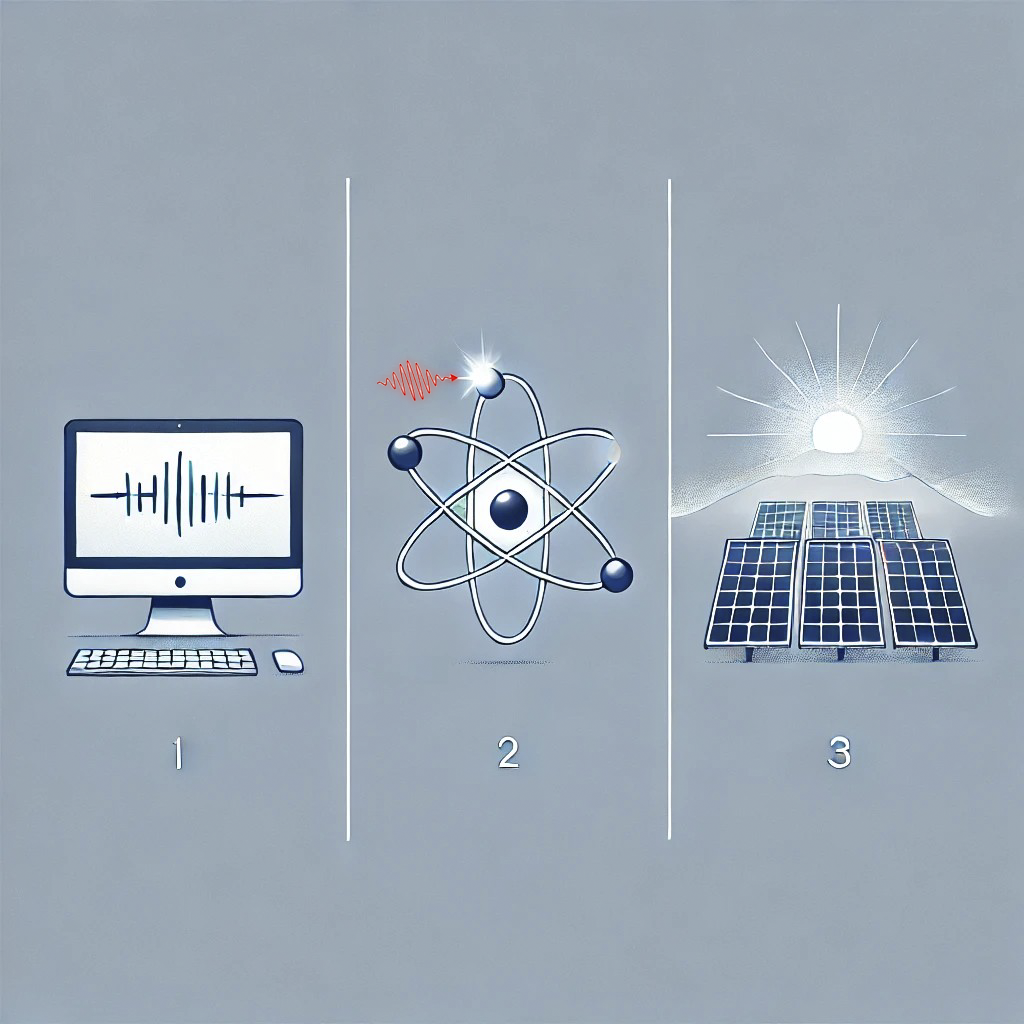
\includegraphics[width=0.48\textwidth]{picture.png}
   \caption{Impact of computational development.}
   \label{fig:fig1}
\end{wrapfigure}
Therefore, figure \ref{fig:fig1} shows how (1) the development of computational methodologies can (2) aid in the spectroscopy of materials to (3) produce more efficient solar cells. Density Functional Theory (DFT) has long served as the go-to computational method in materials science, due to its reasonable accuracy at low computational expense. However, it treats the repulsive interactions between electrons using an approximate exchange-correlation functional, leading to variable results with a lack of systematic improvability \cite{kozlowski_elucidating_2021}. A potential solution is the application of Green's functions in many-body perturbation theory (MBPT). Central is the Dyson equation,
\begin{equation}
G = G_0 + G_0 \Sigma G,
\label{eqn:dyson}
\end{equation}
which relates the Green's function of the fully interacting system \( G \) to that of the non-interacting system \( G_0 \) through the self-energy \( \Sigma \), which is designed to capture the many-body interactions neglected by \( G_0 \). Hedin provided a closed set of 5 equations that can be used to obtain \( G \) and \( \Sigma \). In the common \( GW \) approximation of Hedin's framework, the self-energy \( \Sigma \) takes the form \( iGW \), where \( W \) is the screened Coulomb interaction. Various levels of self-consistency can be done within \( GW \). The most basic is the one-shot \( G_0W_0 \), where the self-energy is calculated using the non-interacting Green's function and the bare Coulomb potential, i.e., \( \Sigma = iG_0W_0 \). Surprisingly, \( G_0W_0 \) has been shown to be quite accurate even at a modest computational cost, due to a fortuitous cancellation of errors. However, it shows a strong starting point dependence on \( G_0 \), which again implies the lack of systematic improvability. At the other extreme, we have fully self-consistent \( GW \) (scGW). Even at the high computational expense necessitated by full self-consistency, this scheme often does not deliver improved results over \( G_0W_0 \). To remedy this, one has to include vertex corrections beyond the \( GW \) approximation within Hedin's framework \cite{kutepov_one-electron_2017}, which is computationally intensive. The root of these issues is that Hedin's equations solve for the self-energy \( \Sigma \) through a perturbative expansion in the interaction strength \( W \). The \( GW \) approximation is accurate for weakly correlated systems where this expansion is reasonable, but it is not for the strongly correlated, where the interaction is large.

The Mori-Zwanzig (MZ) theory offers an alternative. Originating from statistical physics, one starts from a similar Dyson equation \ref{eqn:dyson}, but the self-energy \( \Sigma \) is replaced by a memory kernel. This memory kernel is expanded in powers of the evolution time \( t \), whereas in \( GW \) the self-energy is expanded in powers of the interaction strength \( W \). This makes the series expansion of Dyson's equation converge faster with MZ for strongly correlated systems. Recently, a diagrammatic theory for MZ has been introduced in the form of tree diagrams \cite{zhu_combinatorial_2022}, as opposed to the Feynman diagrams of \( GW \), suggesting the potential for a computational implementation. However, this has not been done yet and is the goal of the proposed work. 

\section*{Research Plan:}
\begin{enumerate}[label=\textbf{Aim \arabic*}]
    \item The uniform electron gas (UEG) is a paradigmatic system in condensed matter physics. As part of my rotation project with Prof. Lee, I am implementing fully self-consistent $GW$ (scGW) for the UEG. Now, I do not have prior experience with the UEG or scGW. However, in past research, I ran quantum chemistry calculations on a periodic system, like the UEG, and completed a senior thesis project on the $G_0W_0$ method within the same $GW$ approximation that scGW follows. I will first corroborate the reported result \cite{holm_fully_1998}, where scGW misses a satellite peak in the frequency spectrum found by highly accurate Quantum Monte Carlo (QMC) simulations.
    \item In the literature, expensive vertex corrections going beyond the $GW$ approximation have been shown to reproduce this satellite peak. I will see if MZ offers a cheaper solution, comparing the number of terms in its perturbative expansion needed to achieve an accuracy on par with vertex-corrected $GW$ for the UEG. I am prepared to work with the MZ theory of open quantum systems from experience with a recent class on quantum many body physics, where I learned to apply matrix product state ideas, culminating in my implementation of the Time Block Evolution Decimation (TEBD) algorithm. More generally, this exploration of MZ on the UEG will enable me to draw connections between MZ and $GW$ for solids, building upon previous work connecting diagrams between $GW$ and wave function-based methods for molecules \cite{Lange_2018}.

    \item I will apply the MZ framework to a realistic condensed matter system. The UEG is known to provide a good description of the Fermi sea in metallic systems, so the transition should be natural. The eventual goal is to study strongly correlated semiconductors composing photovoltaic systems with the MZ framework.
\end{enumerate}

\section*{Motivation and Intellectual Merit:}
The proposed research will develop a computational implementation of the theoretical MZ framework. Much thought has been put into improving upon the $GW$ approximation; this will investigate a hitherto unexplored alternative with the potential to upend how MBPT is done for strongly correlated systems. This work will improve upon traditional ab initio core spectroscopy techniques, enabling the design of improved photovoltaic materials.

\section*{Broader Impacts:}
The proposed research will develop a computational implementation of the theoretical MZ framework. Much thought has been put into improving upon the $GW$ approximation; this will investigate a hitherto unexplored alternative with that potential to upend how MBPT is done for strongly correlated systems. This work will improve upon traditional ab initio core spectroscopy techniques, enabling the design of improved photovoltaic materials.

\bibstyle{plainnat}
\bibliography{citations.bib}

\end{document}

% -------------------------------------------------------------

% -------------------------------------------------------------

